\documentclass[11pt]{article}

\usepackage[margin=1in]{geometry}
\usepackage{iftex}
\ifXeTeX
  \usepackage{fontspec}
  \setmainfont{Latin Modern Roman}
  \usepackage{xeCJK}
  \setCJKmainfont{Noto Serif CJK SC}
  \setCJKsansfont{Noto Sans CJK SC}
  \setCJKmonofont{Noto Sans Mono CJK SC}
  \newCJKfontfamily\zhfont{Noto Serif CJK SC}
\else\ifLuaTeX
  \usepackage{fontspec}
  \setmainfont{Latin Modern Roman}
  \usepackage{luatexja-fontspec}
  \setmainjfont{Noto Serif CJK SC}
  \newjfontfamily\zhfont{Noto Serif CJK SC}
\else
  \usepackage[T1]{fontenc}
  \usepackage{lmodern}
\fi\fi
\usepackage{microtype}
\usepackage{amsmath,amssymb,amsthm,mathtools}
\usepackage{booktabs,array,longtable,tabularx}
\usepackage[dvipsnames]{xcolor}
\usepackage{graphicx}
\usepackage{tikz}
\usetikzlibrary{arrows.meta,positioning,calc,shapes.geometric}
\usepackage[numbers,sort&compress]{natbib}
\usepackage{hyperref}
\usepackage{xurl}
\usepackage{enumitem}
\usepackage{caption}
\usepackage{xspace}

\definecolor{FlowBlue}{HTML}{0072B2}
\definecolor{FlowTeal}{HTML}{009E73}
\definecolor{FlowOrange}{HTML}{E69F00}
\definecolor{FlowRed}{HTML}{D55E00}

\hypersetup{
  colorlinks=true,
  linkcolor=MidnightBlue,
  citecolor=ForestGreen,
  urlcolor=BrickRed,
  pdftitle={The Canonical Koopman Lift Is Too Large},
  pdfauthor={Liang Wang}
}
\urlstyle{same}
\setlength{\emergencystretch}{3em}

\newtheorem{theorem}{Theorem}
\newtheorem{proposition}[theorem]{Proposition}
\newtheorem{corollary}[theorem]{Corollary}
\newtheorem{lemma}[theorem]{Lemma}
\theoremstyle{definition}
\newtheorem{definition}[theorem]{Definition}
\theoremstyle{remark}
\newtheorem{remark}[theorem]{Remark}

\newcommand{\R}{\mathbb{R}}
\newcommand{\Q}{\mathbb{Q}}
\newcommand{\Z}{\mathbb{Z}}
\newcommand{\N}{\mathbb{N}}
\newcommand{\F}{\mathbb{F}}
\newcommand{\C}{\mathbb{C}}
\newcommand{\Hh}{\mathcal{H}}
\newcommand{\D}{\mathcal{D}}
\newcommand{\Tr}{\operatorname{Tr}}
\newcommand{\Ran}{\operatorname{Ran}}
\newcommand{\e}{\mathrm{e}}
\newcommand{\proved}{\textsf{PROVED}\xspace}
\newcommand{\nottest}{\textsf{NOT INVOKED}\xspace}
\newcommand{\failed}{\textsf{FAIL}\xspace}
\newcolumntype{Y}{>{\raggedright\arraybackslash}X}

\title{\textbf{The Canonical Koopman Lift Is Too Large:}\\
Dense Rational Spectrum for a Frobenius Suspension}
\author{Liang Wang\\
\small School of Artificial Intelligence and Automation,\\[-2pt]
\small Huazhong University of Science and Technology, Wuhan 430074, P.R. China\\
\small \texttt{wangliang.f@gmail.com}}
\date{13 August 2026}

\begin{document}
\maketitle

\begin{abstract}
An exact periodic-orbit zeta does not ensure that the canonical unitary lift
of the same flow has a locally finite spectral determinant.  We audit the
unchanged constant-roof \(\log2\) suspension of the square-map Frobenius
\(F(a)=a^2\) on the discrete geometric points of
\(\mathbb P^1_{\mathbb F_2}\).  On the Hilbert
direct sum of its closed-point circles, Koopman translations form a strongly
continuous unitary group whose self-adjoint Stone generator is
\(A_K=\bigoplus_x(-i\,d/du)_{\mathrm{per}}\) on the full periodic Sobolev
domain.  Every family of finite, strictly positive component weights gives a
unitarily equivalent representation.  We prove
\[
 \sigma_{\mathrm p}(A_K)=\frac{2\pi}{\log2}\mathbb Q,
 \qquad
 \sigma(A_K)=\sigma_{\mathrm{ess}}(A_K)=\mathbb R,
\]
and every point eigenvalue has countably infinite multiplicity.  The
eigenvectors nevertheless form a complete pure-point basis; irrational reals
are continuous-spectrum accumulation points in the operator-theoretic set
decomposition, not a continuous part of the vector spectral measures.  The
resolvent is noncompact, every interval of positive width has infinite
spectral-projection rank, and the Gaussian and absolute-value heat operators
are not trace class, even after removal of the zero modes.  Thus the natural
lift passes complete-definition and self-adjointness tests but fails the
local-finiteness gate.  The primitive-orbit Hasse--Weil product and Deligne's
finite-dimensional cohomological Frobenius determinant belong to different
operator ledgers and are not spectral determinants of this generator.
\end{abstract}

\ifPDFTeX\else
\begin{center}
{\zhfont\bfseries 摘要}
\end{center}
{\zhfont
一个精确的周期轨道 zeta 函数，并不保证同一流的典范酉提升具有局部有限
的谱行列式。本文审计一个完全冻结的对象：离散化的
\(\mathbb P^1_{\mathbb F_2}\) 几何点上的算术 Frobenius，以 \(\log2\)
为常值屋顶构造悬挂流。闭点圆周的 Hilbert 直和上，Koopman 平移构成强连续
酉群；其 Stone 自伴生成元为
\(A_K=\bigoplus_x(-i\,d/du)_{\mathrm{per}}\)，定义域是完整的周期 Sobolev
直和定义域。任意严格正且有限的分量权重都与典范测度酉等价。本文证明
点谱恰为 \((2\pi/\log2)\mathbb Q\)，每个点特征值均具有可数无穷重数，且
全谱与本质谱均为 \(\mathbb R\)。特征向量构成完备纯点基，但无理数仍是
算子集合分解意义下的连续谱聚点；这不意味着向量谱测度含连续部分。由此，
预解算子不紧，每个正宽区间的谱投影均为无穷秩，\(e^{-tA_K^2}\) 与
\(e^{-t|A_K|}\) 均非迹类；删除零模后结论仍不改变。因此，该自然提升通过
完整算子定义与自伴性检验，却在局部有限性门槛处严格失败。轨道
Hasse--Weil 乘积及 Deligne 的有限维上同调 Frobenius 行列式属于不同算子
账本，不能被改称为此 Koopman 生成元的谱行列式。
}
\fi

\medskip
\noindent\textbf{Keywords:} Koopman group; Frobenius suspension; Stone
generator; dense point spectrum; essential spectrum; compact resolvent;
Hasse--Weil zeta.

\section{Introduction}
\label{sec:introduction}

The canonical Hilbert-space lift of the frozen Frobenius suspension exists,
is natural, and is self-adjoint.  It is also too large for a locally finite
spectral interpretation.  This combination is useful: it converts an
apparently promising Route-A unitary construction into an exact obstruction
at the first Route-B spectral gate where local eigenvalue counting matters.

Koopman's representation of a measure-preserving dynamics by composition
operators is classical \citep{Koopman1931}.  A measurable flow with invariant
measure gives a one-parameter group of such operators, and strong continuity
places the group under Stone's theorem \citep{Stone1932,TerElstLemanczyk2017}.
The question here is not whether some self-adjoint operator can be written
down.  It is whether the operator forced by an already locked arithmetic flow
has the spectral type required for the determinant aspirations that motivate
arithmetic-flow research.

The underlying flow is the constant-roof suspension of the square-map
Frobenius \(F(a)=a^2\) on \(\mathbb P^1/\F_2\), previously established as a
finite-field positive control \citep{WangFrobenius2026}.  Its primitive orbit
product is
\[
 \prod_{x\in|\mathbb P^1_{\F_2}|}
   \bigl(1-\e^{-s\deg(x)\log2}\bigr)^{-1}
 =\frac{1}{(1-2^{-s})(1-2^{1-s})}.
\]
No roof, phase, potential, component coupling, or fitted coefficient is added
in the present paper.  The sole new step is the canonical Koopman lift on the
same circles with the same clock.

The main result is a complete spectral classification.  Every degree occurs
among the closed points of \(\mathbb P^1/\F_2\).  A degree-\(d\) circle has
Fourier frequencies \(2\pi n/(d\log2)\), so all denominators occur.  More
strongly, a rational frequency \(a/b\) is repeated on degrees \(kb\) at modes
\(ka\) for every \(k\geq1\).  The point spectrum is therefore dense and every
point eigenspace is countably infinite-dimensional.  The direct-sum spectrum
and essential spectrum are both \(\R\).

These facts settle the standard compactness questions without asymptotic
estimates.  The infinite zero eigenspace already prevents compact resolvent
and trace-class heat.  Removing it does not help, because any nonzero rational
frequency has the same infinite multiplicity.  Every interval of positive
width contains such a frequency.  A singleton irrational set, by contrast,
has zero spectral projection; the interval qualifier is essential.

The result also resolves a ledger ambiguity.  The Koopman generator acts on
Fourier modes of \(L^2\) observables.  The orbit product counts primitive
circles and repetitions.  Deligne's formula acts on finite-dimensional
\(\ell\)-adic cohomology \citep{Deligne1974}.  Their common closed-point source
does not provide an intertwiner, trace identity, or determinant identity.
The same-object discipline developed in the companion trace audit forbids
combining coordinates from these separate ledgers \citep{WangTraceBridge2026}.

In the route vocabulary used by the research program, the paper proves
\path{A4_UNITARY_OR_SCATTERING_CANDIDATE},
\path{B1_COMPLETE_OPERATOR_DEFINITION}, and
\path{B2_SELF_ADJOINT}; it also proves \path{B3_FAIL}.  The scoped
result is \path{ROUTE_B_REJECTED} at Gate C.  B4 and B5 are outside this
limited audit and receive no verdict.  No Hilbert--P\'olya claim is made.

\begin{figure}[t]
  \centering
  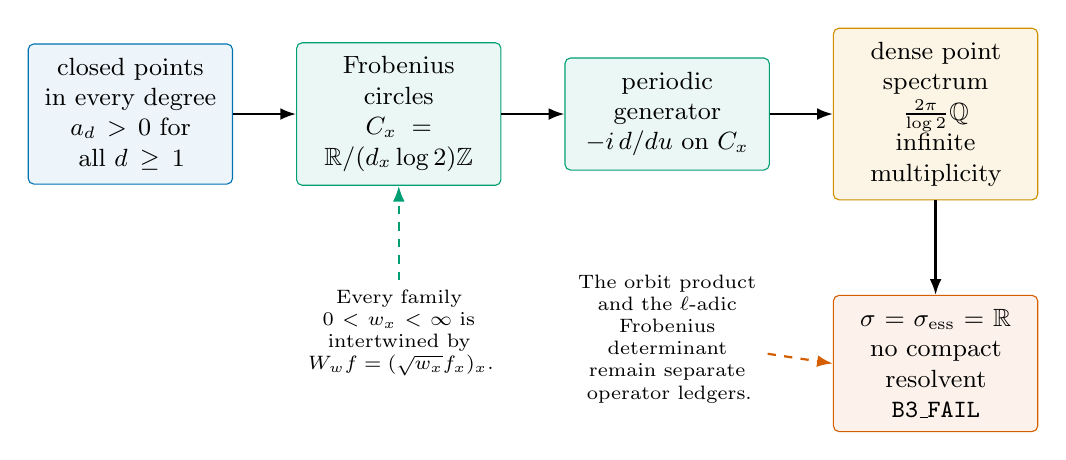
\begin{tikzpicture}[
  node distance=7mm and 8mm,
  box/.style={draw,rounded corners=2pt,align=center,inner sep=5pt,
              text width=0.185\textwidth,minimum height=12mm,font=\small},
  source/.style={box,draw=FlowBlue,fill=FlowBlue!7},
  op/.style={box,draw=FlowTeal,fill=FlowTeal!8},
  result/.style={box,draw=FlowOrange!90!black,fill=FlowOrange!10},
  fail/.style={box,draw=FlowRed,fill=FlowRed!8},
  arr/.style={-{Latex[length=2mm]},thick},
  note/.style={font=\scriptsize,align=center,text width=0.19\textwidth}
]
\node[source] (degrees) {closed points in every degree\\$a_d>0$ for all $d\geq1$};
\node[op,right=of degrees] (circles) {Frobenius circles\\$C_x=\R/(d_x\log2)\Z$};
\node[op,right=of circles] (fourier) {periodic generator\\$-i\,d/du$ on $C_x$};
\node[result,right=of fourier] (rational) {dense point spectrum\\$\frac{2\pi}{\log2}\Q$\\infinite multiplicity};
\node[fail,below=12mm of rational] (b3) {$\sigma=\sigma_{\rm ess}=\R$\\no compact resolvent\\\texttt{B3\_FAIL}};

\draw[arr] (degrees) -- (circles);
\draw[arr] (circles) -- (fourier);
\draw[arr] (fourier) -- (rational);
\draw[arr] (rational) -- (b3);

\node[note,below=12mm of circles] (weights) {Every family $0<w_x<\infty$ is intertwined by\\$W_wf=(\sqrt{w_x}f_x)_x$.};
\draw[arr,dashed,FlowTeal] (weights) -- (circles);

\node[note,below=12mm of fourier] (ledger) {The orbit product and the \(\ell\)-adic Frobenius determinant remain separate operator ledgers.};
\draw[arr,dashed,FlowRed] (ledger) -- (b3.west);
\end{tikzpicture}

  \caption{Exact implication chain for the frozen Koopman candidate.  The
  positive-weight family is one unitary-equivalence class, while the orbit and
  cohomological ledgers do not become determinants of the Stone generator.}
  \label{fig:obstruction}
\end{figure}

\section{The frozen Frobenius suspension}
\label{sec:frozen}

Let
\[
 X=\mathbb P^1_{\F_2},\qquad
 S=X(\overline{\F}_2)_{\mathrm{disc}},\qquad
 F(a)=a^2,\qquad \tau=\log2.
\]
The topology on \(S\) is explicitly discrete.  It is a modeling choice
inherited from the frozen classical candidate, not a topology of the scheme.
We call \(F(a)=a^2\) the square-map Frobenius convention throughout.  Sources
that place geometric and arithmetic Frobenius inversely may use the opposite
name.  Replacing \(F\) by \(F^{-1}\) only reverses each finite cycle and leaves
its degree, suspension length, and every spectrum calculation below
unchanged; the frozen return map itself remains \(a\mapsto a^2\).
The mapping torus and vertical flow are
\begin{equation}
 M_F=(S\times\R)/\Z,
 \qquad n\cdot(a,u)=(F^na,u-n\tau),
 \qquad \phi^t[a,u]=[a,u+t].
 \label{eq:mapping-torus}
\end{equation}
Closed points are the finite Frobenius orbits on geometric points
\citep[Sec.~1.4]{Deligne1974}.  If \(x\) has residue degree \(d_x\), its
suspension component is the circle
\begin{equation}
 C_x=\R/(L_x\Z),\qquad L_x=d_x\log2,
 \qquad
 M_F\cong\coprod_{x\in|X|}C_x .
 \label{eq:circle-decomposition}
\end{equation}
The flow on \(C_x\) is \(u\mapsto u+t\pmod{L_x}\).  Each component is open
and closed, and the component set is countable.

The orbit identity quoted in the Introduction belongs to the classical
ledger.  It comes from the bijection between closed points and primitive
circles and from the period identity
\(L_x=\deg(x)\log2=\log N(x)\).  The present operator construction changes
none of these data.  Table~\ref{tab:operator-lock} records every new analytic
choice before the spectral calculation.

\begin{table}[t]
\centering
\caption{Frozen definition of candidate
\texttt{FF-FROB-SUSP-P1-F2-KOOPMAN-P1}.}
\label{tab:operator-lock}
\small
\begin{tabularx}{\textwidth}{@{}p{0.25\textwidth}YY@{}}
\toprule
Field & Canonical representative & Allowed equivalent family\\
\midrule
Components & \(C_x=\R/(d_x\log2)\Z\) & unchanged\\
Measure & \(\mu_1|_{C_x}=du_x\) & \(\mu_w|_{C_x}=w_xdu_x\), \(0<w_x<\infty\)\\
Hilbert space & \(\bigoplus_x^2L^2(C_x,du_x)\) & \(\bigoplus_x^2L^2(C_x,w_xdu_x)\)\\
Group & \((U_tf)_x(u)=f_x(u-t)\) & same formula\\
Stone convention & \(U_t=\e^{-itA_K}\) & same convention\\
Component action & \(-i\,d/du\) & same action\\
Boundary condition & periodic Sobolev trace & unchanged\\
Added data & none & positive constants only\\
\bottomrule
\end{tabularx}
\end{table}

\section{A closed point in every degree}
\label{sec:degrees}

The later spectral result needs only one component of each positive degree.
For completeness, the exact degree count is recorded first.  Let \(a_d\) be
the number of degree-\(d\) closed points of \(X\).  The affine closed points
are monic irreducible polynomials over \(\F_2\), whose number is given by the
standard M\"obius formula \citep[Thm.~1.3.6]{NiederreiterXing2009}.  The point
at infinity adds one degree-one point, hence
\begin{equation}
 a_1=3,
 \qquad
 a_d=\frac1d\sum_{e\mid d}\mu_{\mathrm{Mob}}(e)2^{d/e}
 \quad(d\geq2).
 \label{eq:closed-point-count}
\end{equation}

\begin{lemma}[Degree support]
\label{lem:degree-support}
For every \(d\geq1\), \(a_d>0\).
\end{lemma}

\begin{proof}
The degree-one claim follows from \(0,1,\infty\).  If \(d\geq2\), then
\begin{align*}
 d a_d
 &=2^d+\sum_{\substack{e\mid d\\e\geq2}}
       \mu_{\mathrm{Mob}}(e)2^{d/e}\\
 &\geq2^d-\sum_{\substack{e\mid d\\e\geq2}}2^{d/e}
 \geq2^d-\sum_{j=1}^{\lfloor d/2\rfloor}2^j\\
 &=2^d-2^{\lfloor d/2\rfloor+1}+2>0.
\end{align*}
The last expression equals \(2\) when \(d=2\) and is positive thereafter.
\end{proof}

The exponential size of \(a_d\) is not used below.  The assertion
\(a_d\geq1\) for each degree is already enough to generate dense point
spectrum and infinite multiplicity.  Thus deleting all but one closed point
in every degree would not repair the obstruction, although that deletion
would define a different classical object.

\section{Invariant measures and one Hilbert class}
\label{sec:measures}

The canonical measure is counting measure on the discrete base times
Lebesgue flow time, passed to the quotient.  On the circle decomposition it
is simply
\[
 \mu_1=\sum_xdu_x.
\]
More generally, fix any family \(w=(w_x)_x\) with
\(0<w_x<\infty\), and put
\begin{equation}
 \mu_w=\sum_xw_xdu_x,
 \qquad
 \Hh_w=L^2(M_F,\mu_w)
 =\bigoplus_x^{\,2}L^2(C_x,w_xdu_x).
 \label{eq:weighted-space}
\end{equation}

\begin{proposition}[Measure properties]
\label{prop:measure}
Every \(\mu_w\) is invariant, sigma-finite, Radon, and has full support.
\end{proposition}

\begin{proof}
Translation preserves \(du_x\), hence every constant multiple
\(w_xdu_x\).  The component set is countable and each circle has finite
weighted measure, proving sigma-finiteness.  Strict positivity gives positive
measure to every nonempty open subset of each component, so the measure has
full support.  A compact subset of a topological coproduct meets only finitely
many open-and-closed components.  Its measure is therefore a finite sum of
finite circle measures, which proves the Radon property.
\end{proof}

\begin{theorem}[Positive-weight unitary equivalence]
\label{thm:weight-equivalence}
Define
\begin{equation}
 W_w:\Hh_w\longrightarrow\Hh_1,
 \qquad (W_wf)_x=\sqrt{w_x}\,f_x.
 \label{eq:weight-intertwiner}
\end{equation}
Then \(W_w\) is unitary and intertwines the Koopman groups.  After the
generators are defined in Section~\ref{sec:generator}, it also maps their
domains onto one another and satisfies \(W_wA_w=A_1W_w\).
\end{theorem}

\begin{proof}
The norm identity
\[
 \|W_wf\|_{\Hh_1}^2
 =\sum_x\int_{C_x}w_x|f_x|^2du_x
 =\|f\|_{\Hh_w}^2
\]
holds, and componentwise multiplication by \(w_x^{-1/2}\) is the inverse.
Constant multiplication commutes with translation and differentiation.  The
same identity applied to \(f_x'\) proves the graph-norm and domain assertions.
\end{proof}

Choosing positive weights with \(\sum_xw_xL_x=1\) makes \(\mu_w\) a
probability measure, and \(w_x=L_x^{-1}\) gives normalized Haar measure on
every component.  Both are in the same unitary class.  A zero component
weight is excluded: it deletes closed-point data and is therefore a new
candidate, not a reweighting.

\section{Koopman group and self-adjoint generator}
\label{sec:generator}

Freeze the inverse-flow pullback convention
\begin{equation}
 (U_t^{(w)}f)_x(u)=f_x(u-t),
 \qquad U_t^{(w)}=\e^{-itA_w}.
 \label{eq:koopman-group}
\end{equation}
The measure invariance in Proposition~\ref{prop:measure} gives unitarity.
This is the usual Koopman construction for a measure-preserving flow
\citep{TerElstLemanczyk2017}.

\begin{proposition}[Strong continuity]
\label{prop:strong-continuity}
The family \((U_t^{(w)})_{t\in\R}\) is a strongly continuous unitary group.
\end{proposition}

\begin{proof}
Translation is strongly continuous on each circle \(L^2\)-space.  Given
\(f\in\Hh_w\) and \(\varepsilon>0\), choose a vector \(g\), supported on
finitely many components, with \(\|f-g\|<\varepsilon\).  Then
\[
 \|U_t^{(w)}f-f\|
 \leq2\|f-g\|+\|U_t^{(w)}g-g\|.
\]
The last term tends to zero in a finite direct sum.  Since \(\varepsilon\)
is arbitrary, the claim follows.
\end{proof}

The formal derivative is insufficient until its domain and boundary
conditions are fixed.  Define
\begin{equation}
 A_w=\bigoplus_xA_x,
 \qquad A_x=-i\frac d{du},
 \label{eq:global-generator}
\end{equation}
on
\begin{equation}
\begin{split}
 \D(A_w)=\bigg\{f=(f_x):\;&
 f_x\in H^1_{\mathrm{per}}(0,L_x)\text{ for every }x,\\
 &\sum_xw_x\bigl(\|f_x\|_{L^2(du_x)}^2
                  +\|f_x'\|_{L^2(du_x)}^2\bigr)<\infty\bigg\}.
\end{split}
\label{eq:generator-domain}
\end{equation}
The periodic condition means \(f_x(0)=f_x(L_x)\) in the Sobolev trace
sense.

\begin{theorem}[Complete operator and Stone generator]
\label{thm:self-adjoint}
The operator \(A_w\) on \eqref{eq:generator-domain} is self-adjoint and is
the unique Stone generator of \eqref{eq:koopman-group}.  Finite-component
trigonometric polynomials form a core.
\end{theorem}

\begin{proof}
Periodic Fourier transform gives the normalized component basis
\begin{equation}
 e_{x,n}^{(w)}(u)=(w_xL_x)^{-1/2}\e^{2\pi inu/L_x},
 \qquad n\in\Z,
 \label{eq:fourier-basis}
\end{equation}
and
\begin{equation}
 A_xe_{x,n}^{(w)}=\frac{2\pi n}{L_x}e_{x,n}^{(w)}.
 \label{eq:component-frequency}
\end{equation}
Thus \(A_x\) is unitarily equivalent to multiplication by the real sequence
\((2\pi n/L_x)_{n\in\Z}\) on its maximal domain, which is precisely periodic
\(H^1\).  It is self-adjoint.  The orthogonal-sum theorem now gives a
self-adjoint global operator on the maximal graph-summability domain
\eqref{eq:generator-domain} \citep[Thm.~2.23]{Teschl2009}.

Componentwise exponentiation produces translations.  The sign is fixed by
\[
 \left.\frac d{dt}U_t^{(w)}f\right|_{t=0}=-f'
 =-i\left(-i\frac d{du}\right)f.
\]
Stone's theorem gives uniqueness \citep{Stone1932,Teschl2009}.  Finite
component truncation followed by finite Fourier truncation converges in the
global graph norm, proving the core statement.
\end{proof}

Theorem~\ref{thm:self-adjoint} establishes the two positive limited-route
facts: \path{B1_COMPLETE_OPERATOR_DEFINITION} and
\path{B2_SELF_ADJOINT}.

\section{Exact point spectrum and degeneracy}
\label{sec:point-spectrum}

\begin{theorem}[Point spectrum]
\label{thm:point-spectrum}
For every positive weight family,
\begin{equation}
 \boxed{\displaystyle
 \sigma_{\mathrm p}(A_w)=\frac{2\pi}{\log2}\Q.}
 \label{eq:point-spectrum}
\end{equation}
\end{theorem}

\begin{proof}
A degree-\(d\) component has, by \eqref{eq:component-frequency}, the
frequency lattice
\[
 \frac{2\pi}{d\log2}\Z.
\]
Lemma~\ref{lem:degree-support} supplies at least one component for every
positive \(d\), and the union of these lattices is
\((2\pi/\log2)\Q\).

Conversely, suppose \(A_wf=\lambda f\) with \(f\neq0\).  At least one
component \(f_x\) is nonzero, and it satisfies \(A_xf_x=\lambda f_x\).
The component Fourier diagonalization forces
\(\lambda=2\pi n/(d_x\log2)\) for some \(n\in\Z\).  No other eigenvalues
occur.
\end{proof}

\begin{theorem}[Countably infinite multiplicity]
\label{thm:multiplicity}
Every \(\lambda\in\sigma_{\mathrm p}(A_w)\), including zero, has countably
infinite multiplicity.
\end{theorem}

\begin{proof}
Write \(\lambda=(2\pi/\log2)(a/b)\), with \(a/b\) in lowest terms and
\(b\geq1\).  For every \(k\geq1\), choose a closed point \(x_k\) of degree
\(kb\), possible by Lemma~\ref{lem:degree-support}, and take Fourier mode
\(ka\).  Then
\begin{equation}
 A_we_{x_k,ka}^{(w)}
 =\frac{2\pi}{\log2}\frac ab\,e_{x_k,ka}^{(w)}.
 \label{eq:multiplicity-witness}
\end{equation}
The vectors have disjoint component supports and are orthonormal.  For
\(a=0\), the same construction is the constant mode on one component in each
degree.  Multiplicity is at most countable because the complete Fourier basis
is countable.
\end{proof}

The mechanism is not the large value of \(a_d\).  One point in every degree
already provides the sequence \((kb,ka)\).  Nor is it restricted to invariant
functions: when \(a\neq0\), every witness in
\eqref{eq:multiplicity-witness} is a nonconstant Fourier mode.

\section{Full spectrum, essential spectrum, and terminology}
\label{sec:full-spectrum}

\begin{theorem}[Global spectral classification]
\label{thm:global-spectrum}
For every positive component-weight family,
\begin{equation}
 \boxed{\displaystyle
 \sigma(A_w)=\sigma_{\mathrm{ess}}(A_w)=\R,
 \qquad \sigma_{\mathrm{disc}}(A_w)=\varnothing.}
 \label{eq:global-spectrum}
\end{equation}
\end{theorem}

\begin{proof}
The spectrum of a countable orthogonal sum is the closure of the union of
the component spectra \citep[Thm.~2.23]{Teschl2009}.  Theorem
\ref{thm:point-spectrum} and density of \(\Q\) give
\[
 \sigma(A_w)=\overline{(2\pi/\log2)\Q}=\R.
\]
Every neighborhood of a rational spectral point contains its
infinite-dimensional eigenspace.  If \(\lambda\) is irrational, choose
distinct rational frequencies \(\lambda_j\to\lambda\), and choose their
normalized eigenvectors on mutually distinct components.  Then
\[
 \|(A_w-\lambda)e_j\|=|\lambda_j-\lambda|\longrightarrow0,
 \qquad e_j\rightharpoonup0.
\]
This is a singular Weyl sequence.  Hence every real point is essential, and
no isolated finite-multiplicity eigenvalue remains in the discrete spectrum
\citep[Secs.~6.2--6.4]{Teschl2009}.
\end{proof}

\begin{remark}[Two meanings that must not be conflated]
\label{rem:pure-point}
The set \(\{e_{x,n}^{(w)}\}_{x,n}\) is a complete orthonormal eigenbasis, so
every vector spectral measure is atomic, or pure point.  At the same time,
the operator-theoretic set decomposition is
\begin{equation}
 \sigma_{\mathrm p}(A_w)=\frac{2\pi}{\log2}\Q,
 \qquad
 \sigma_{\mathrm c}(A_w)=
 \R\setminus\frac{2\pi}{\log2}\Q,
 \qquad \sigma_{\mathrm r}(A_w)=\varnothing.
 \label{eq:spectral-types}
\end{equation}
For an irrational \(\lambda\), \(A_w-\lambda\) is injective with dense but
nonsurjective range.  Such points are continuous-spectrum accumulation points
as a subset of the operator spectrum.  They do not create a continuous
component in any vector spectral measure.  A complete pure-point basis is
therefore compatible with dense spectrum and empty compact-resolvent discrete
spectrum.
\end{remark}

\section{Compactness, counting, and heat obstructions}
\label{sec:obstructions}

The global spectral theorem gives the exact Route-B obstruction.

\begin{proposition}[Noncompact resolvent]
\label{prop:resolvent}
For every \(z\in\C\setminus\R\), \((A_w-z)^{-1}\) is not compact.  The
failure remains on the orthogonal complement of \(\ker A_w\).
\end{proposition}

\begin{proof}
On every normalized zero mode,
\[
 (A_w-z)^{-1}e_{x,0}^{(w)}=-z^{-1}e_{x,0}^{(w)}.
\]
The resolvent sends an infinite orthonormal sequence to a fixed nonzero
multiple of itself, whose image has no norm-convergent subsequence.  After
deleting the kernel, choose any nonzero rational eigenvalue \(\lambda\).
Theorem~\ref{thm:multiplicity} supplies an infinite orthonormal set on which
the reduced resolvent is multiplication by \((\lambda-z)^{-1}\).
\end{proof}

\begin{proposition}[No locally finite eigenvalue count]
\label{prop:counting}
If \(I\subset\R\) is an interval of positive width, then
\begin{equation}
 \operatorname{rank}\mathbf1_I(A_w)=\infty.
 \label{eq:local-rank}
\end{equation}
Consequently
\begin{equation}
 N(E):=\dim\Ran\mathbf1_{[-E,E]}(A_w)=\infty
 \qquad(E\geq0).
 \label{eq:counting-function}
\end{equation}
\end{proposition}

\begin{proof}
Every positive-width interval contains a member of
\((2\pi/\log2)\Q\), and its eigenspace is infinite-dimensional.  For
\(E=0\), the centered projection is the infinite-dimensional kernel.  The
word ``interval'' cannot be replaced by an arbitrary nonempty Borel set: a
singleton irrational set has spectral-projection rank zero.
\end{proof}

\begin{proposition}[No trace-class heat]
\label{prop:heat}
For every \(t>0\), neither \(\e^{-tA_w^2}\) nor \(\e^{-t|A_w|}\) is trace
class.  The same holds after zero-mode deletion.  Moreover,
\((1+A_w^2)^{-s/2}\) is not trace class for any \(s>0\).
\end{proposition}

\begin{proof}
Both heat functions equal one on the infinite zero eigenspace.  After its
removal, fix a nonzero rational eigenvalue \(\lambda\).  Its infinite
eigenspace receives the same positive multiplier \(\e^{-t\lambda^2}\), or
\(\e^{-t|\lambda|}\).  The resolvent power similarly repeats the positive
number \((1+\lambda^2)^{-s/2}\) infinitely.  Each operator is therefore
noncompact and not trace class.
\end{proof}

The symbol \(\e^{-tA_w}\) is not used as a heat operator: \(A_w\) is
unbounded below.  The standard semigroup choices are functions of \(A_w^2\)
or \(|A_w|\), and those already fail.

Bornemann's account of the ordinary operator determinant defines
\(\det(I+zK)\) canonically for trace-class \(K\) and relates the usual product,
Plemelj, and exterior-power descriptions \citep[Secs.~2--3]{Bornemann2010}.
The frozen resolvent, heat functions, and Koopman group do not supply such a
trace-class input.  A compact-resolvent spectral-zeta determinant is also
unavailable because every positive-width window has infinite rank.  This is
a boundary for the standard constructions.  It does not assert that no
relative, compressed, or renormalized determinant can ever be defined; each
would require additional choices and would constitute a new candidate.

\begin{table}[t]
\centering
\caption{Exact theorem ledger for the frozen generator.}
\label{tab:theorem-ledger}
\small
\begin{tabularx}{\textwidth}{@{}p{0.31\textwidth}Yp{0.18\textwidth}@{}}
\toprule
Property & Result & Status\\
\midrule
Point spectrum & \((2\pi/\log2)\Q\) & \proved\\
Point multiplicity & countably infinite at every point eigenvalue & \proved\\
Full and essential spectrum & both equal \(\R\) & \proved\\
Discrete spectrum & empty & \proved\\
Vector spectral measures & pure point; complete eigenbasis & \proved\\
Irrational operator-spectrum points & continuous spectrum, no eigenvectors & \proved\\
Resolvent & noncompact, also after kernel deletion & \proved\\
Positive-width interval projections & infinite rank & \proved\\
Heat and resolvent powers & not trace class & \proved\\
Ordinary generator determinant & standard required inputs unavailable & \proved boundary\\
\bottomrule
\end{tabularx}
\end{table}

\section{Why the orbit zeta is not this spectral determinant}
\label{sec:ledgers}

Three constructions share arithmetic input but not an operator.  The orbit
ledger is
\begin{equation}
 Z_{\mathrm{orb}}(s)
 =\prod_x\bigl(1-\e^{-s d_x\log2}\bigr)^{-1}.
 \label{eq:orbit-ledger}
\end{equation}
It counts one primitive suspension circle per closed point and all positive
repetitions.  The Koopman ledger is
\begin{equation}
 \Hh_w=\bigoplus_x^2L^2(C_x,w_xdu_x),
 \qquad
 A_w=\bigoplus_x(-i\,d/du)_{\mathrm{per}},
 \label{eq:koopman-ledger}
\end{equation}
which counts positive, negative, and zero Fourier modes on every circle.
Nothing in \eqref{eq:orbit-ledger} identifies its repetition coefficients
with a trace of \eqref{eq:koopman-ledger}.

The third ledger is Deligne's alternating cohomological expression
\begin{equation}
 Z(X,t)=\prod_i
 \det\!\left(I-t\Phi_{\mathrm{coh}}\mid
 H_c^i(X_{\overline{\F}_2},\mathbb Q_\ell)\right)^{(-1)^{i+1}},
 \label{eq:cohomological-ledger}
\end{equation}
where \(\Phi_{\mathrm{coh}}\) is the appropriate Frobenius action on
compactly supported \(\ell\)-adic cohomology
\citep[Eq.~(1.5.4)]{Deligne1974}.  These spaces are finite-dimensional in the
present case and have an alternating cohomological grading.  They are not the
circle-observable Hilbert space, and \(\Phi_{\mathrm{coh}}\) is not the
periodic derivative.

\begin{figure}[t]
  \centering
  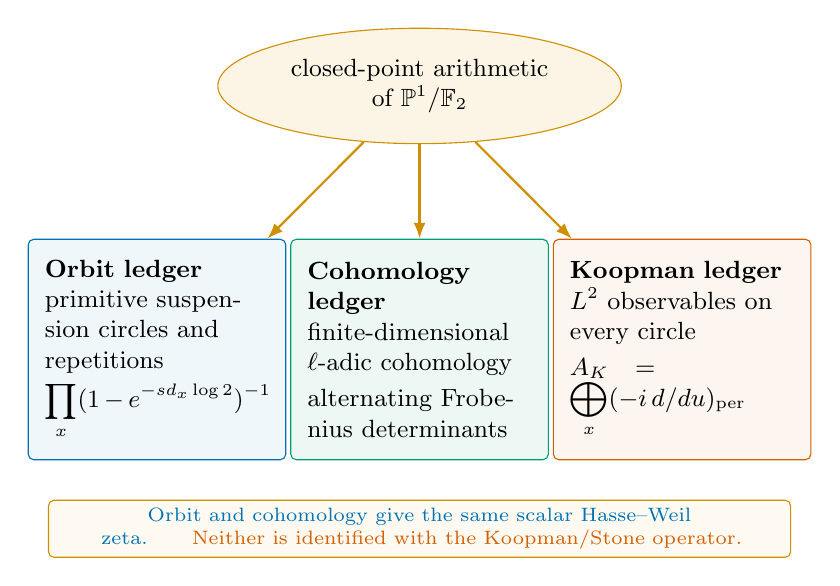
\begin{tikzpicture}[
  node distance=6mm,
  ledger/.style={draw,rounded corners=2pt,align=left,inner sep=6pt,
                 text width=0.235\textwidth,minimum height=28mm,font=\small},
  arr/.style={-{Latex[length=2mm]},thick},
  shared/.style={draw,ellipse,align=center,inner sep=5pt,
                 fill=FlowOrange!10,draw=FlowOrange!90!black,font=\small},
  relation/.style={draw,rounded corners=2pt,align=center,inner sep=3pt,
                   text width=0.76\textwidth,font=\scriptsize}
]
\node[shared] (source) {closed-point arithmetic\\of $\mathbb P^1/\F_2$};
\node[ledger,below=12mm of source,xshift=-0.275\textwidth,draw=FlowBlue,fill=FlowBlue!6] (orbit)
{\textbf{Orbit ledger}\\primitive suspension circles and repetitions\\[2pt]
$\displaystyle\prod_x(1-e^{-s d_x\log2})^{-1}$};
\node[ledger,below=12mm of source,draw=FlowTeal,fill=FlowTeal!7] (coh)
{\textbf{Cohomology ledger}\\finite-dimensional $\ell$-adic cohomology\\[2pt]
alternating Frobenius determinants};
\node[ledger,below=12mm of source,xshift=0.275\textwidth,draw=FlowRed,fill=FlowRed!6] (koop)
{\textbf{Koopman ledger}\\$L^2$ observables on every circle\\[2pt]
$\displaystyle A_K=\bigoplus_x(-i\,d/du)_{\rm per}$};
\draw[arr,FlowOrange!90!black] (source) -- (orbit);
\draw[arr,FlowOrange!90!black] (source) -- (coh);
\draw[arr,FlowOrange!90!black] (source) -- (koop);
\node[relation,below=5mm of coh,draw=FlowOrange!90!black,fill=FlowOrange!5]
{\textcolor{FlowBlue}{Orbit and cohomology give the same scalar
Hasse--Weil zeta.}\qquad
\textcolor{FlowRed}{Neither is identified with the Koopman/Stone operator.}};
\end{tikzpicture}

  \caption{The shared closed-point source explains the scalar agreement of
  the orbit and cohomological Hasse--Weil constructions.  It does not identify
  either operator with the Koopman/Stone generator.}
  \label{fig:ledgers}
\end{figure}

\begin{proposition}[Same-object non-identification]
\label{prop:nonidentification}
The frozen data supply no unitary conjugacy, trace theorem, or determinant
identity between \(A_w\) and the cohomological Frobenius action.  Therefore
the orbit Hasse--Weil zeta cannot be presented as an ordinary Fredholm or
compact-resolvent spectral-zeta determinant of \(A_w\).
\end{proposition}

\begin{proof}
The spaces, actions, and spectral types in
\eqref{eq:koopman-ledger} and \eqref{eq:cohomological-ledger} are explicitly
different.  No bridge morphism is part of the candidate.  Independently,
Propositions~\ref{prop:resolvent}--\ref{prop:heat} show that the standard
trace-class or compact-resolvent inputs fail on the Koopman side.  A scalar
identity derived from common closed-point counts cannot supply the missing
operator map \citep{WangTraceBridge2026}.
\end{proof}

\section{Koopman representation is not a physical quantization}
\label{sec:quantization}

The candidate is a natural unitary representation of classical transport.
It maps an observable \(f\) to its pullback along the flow and converts time
translation into a self-adjoint Stone generator.  This justifies the formal
enum \texttt{A4\_UNITARY\_OR\_SCATTERING\_CANDIDATE}.

Physical or geometric quantization requires further frozen structure.  A
standard geometric-quantization package includes symplectic and prequantum
data together with a polarization or an alternative rule that fixes the
observable-to-operator map \citep{Kostant1970}.  The present disconnected
circle suspension supplies none of those data, no Planck normalization, and
no physical observable assignment beyond Koopman transport.  Accordingly,
the paper does not award \texttt{A4\_NATURAL\_QUANTIZATION} or
\texttt{A4\_ROUTE\_B\_READY}.  This is a statement about the frozen candidate,
not an impossibility theorem for every enrichment or quantization scheme.

\section{Controls, limitations, and route verdict}
\label{sec:controls}

\subsection{Deterministic controls}

The companion standard-library Python program regenerates three finite
control tables and a manifest.  It checks M\"obius degree counts through
degree 24, reconstructs fixed-point counts, verifies finite prefixes of the
degree-\(kb\), mode-\(ka\) witnesses, and tests the weight intertwiner on a
finite Fourier vector.  The control suite ran eight tests, all passing.

\begin{table}[t]
\centering
\caption{Deterministic control suite.  Finite regressions check the
implementation; the infinite claims are proved in the preceding sections.}
\label{tab:controls}
\small
\begin{tabularx}{\textwidth}{@{}p{0.31\textwidth}p{0.19\textwidth}Y@{}}
\toprule
Control & Result & Evidentiary boundary\\
\midrule
Unit tests & 8/8 pass & code and artifact consistency\\
Closed-point counts & positive through degree 24 & regression for Lemma~\ref{lem:degree-support}\\
Fixed-point reconstruction & all rows match & primitive-degree ledger check\\
Frequency witnesses & six signed rationals, 12 witnesses each & finite check of \((kb,ka)\) construction\\
Kernel-deletion witness & survives & nonzero multiplicity control\\
Weight intertwiner & norm error zero; max action error \(2.29\times10^{-16}\) & finite floating-point regression\\
Manifest exclusions & no zeros; no fitted parameters; B4/B5 not invoked & scope lock\\
\bottomrule
\end{tabularx}
\end{table}

The generated manifest is
\path{results/koopman_spectral_manifest.json}.  It records
\texttt{target\_zero\_data\_used: false}, an empty
\texttt{fitted\_parameters} array, and
\texttt{b4\_b5\_invoked: false}.  The run is deterministic, has no random
seed, makes no network request, and reads no rational-prime or target-zero
table.  The command is
\begin{verbatim}
./experiments/reproduce.sh
\end{verbatim}
from the Paper 5 directory.

\subsection{Limitations}

The base topology is an imposed discrete topology inherited from the
classical positive control.  The resulting space is a countable topological
coproduct of neutral periodic circles, with no coupling or transverse
hyperbolicity.  The Koopman conclusion therefore applies to this precise
candidate and its positive component-weight unitary class.  It is not a
no-go theorem for all Frobenius-inspired operators.

The paper analyzes the canonical uncoupled translation representation.
Adding a potential, off-diagonal coupling, nonconstant density, new boundary
condition, compression, finite-degree cutoff, or renormalization changes the
operator and requires a new source and same-object audit.  A finite cutoff
does have compact resolvent, but no frozen cutoff-removal or determinant
renormalization theorem is supplied.

The determinant conclusion is likewise scoped to ordinary Fredholm and
compact-resolvent spectral-zeta mechanisms formed from the frozen generator.
It does not exclude a separately defined relative determinant.  Nor does it
deny Deligne's cohomological determinant, whose correctness is exactly why
the operator ledger must be named precisely.

No Riemann zeros, zero statistics, fitted scale, spectral shift, phase,
potential, or target-informed boundary condition enter the construction or
the controls.  The paper therefore makes no numerical or inferential claim
about a Riemann-zero correspondence.

\subsection{Formal route report}

Table~\ref{tab:route} serializes only the layers actually audited.  B4 and B5
are listed as scope annotations, not as verdict enums.

\begin{table}[t]
\centering
\caption{Route A/A4 and limited Route B/B1--B3 assessment.}
\label{tab:route}
\small
\begin{tabularx}{\textwidth}{@{}p{0.16\textwidth}p{0.43\textwidth}Y@{}}
\toprule
Layer & Formal enum & Result and reason\\
\midrule
A4 & \texttt{A4\_UNITARY\_OR\_SCATTERING\_CANDIDATE} & \proved: canonical same-clock Koopman lift\\
B1 & \texttt{B1\_COMPLETE\_OPERATOR\_DEFINITION} & \proved: space, measure, action, domain, boundary conditions\\
B2 & \texttt{B2\_SELF\_ADJOINT} & \proved: Fourier and orthogonal-sum proof\\
B3 & \texttt{B3\_FAIL} & \proved: dense, infinitely degenerate essential spectrum\\
B4 & outside limited audit & \nottest; no verdict serialized\\
B5 & outside limited audit & \nottest; no verdict serialized\\
Overall & \texttt{ROUTE\_B\_REJECTED} & Gate C; \texttt{hilbert\_polya\_claim\_allowed: false}\\
\bottomrule
\end{tabularx}
\end{table}

The earlier Riemann-target Route-A rejection of the fixed finite-field clock
is unchanged \citep{WangFrobenius2026}.  The successful construction of a
self-adjoint Koopman operator does not repair that classical arithmetic
support mismatch, and B3 independently rejects this operator as a locally
finite spectral host.

\section{Conclusion}

The Frobenius suspension does possess a fixed and natural self-adjoint
Koopman generator.  Its exact spectrum is nevertheless dense and infinitely
degenerate: the point spectrum is \((2\pi/\log2)\Q\), while the full and
essential spectra are \(\R\).  This proves that the generator cannot serve as
the required locally finite determinant host under the standard mechanisms.

Any subsequent trace interface must identify a different source-derived
operator and provide a rigorous same-object morphism.  Transplanting the
Hasse--Weil orbit or cohomological ledger into \(A_K\) would erase precisely
the distinction established here.

\section*{Reproducibility and declarations}

\paragraph{Data and code availability.}
All source-lock notes, acquired-source hashes, proof records, deterministic
Python code, tests, generated CSV controls, JSON manifest, TikZ sources,
bibliography, and manuscript source are included in
\path{papers/5-quantum-flow/}; acquired source artifacts and their SHA-256
hashes are listed in \path{notes/source_matrix.md}.  No external dataset or
target-zero dataset was created or analyzed.

\paragraph{Ethics statement.}
This theoretical and deterministic computational study involves no human
participants, animals, intervention, personal data, or identifiable
information.  Institutional ethics review was not required.

\paragraph{CRediT authorship contribution statement.}
Liang Wang: Conceptualization, Methodology, Formal analysis, Investigation,
Software, Validation, Data curation, Visualization, Writing---original draft,
and Writing---review and editing.

\paragraph{Funding.}
No project-specific external funding source was declared for this work.

\paragraph{Conflict of interest.}
The author declares no financial or non-financial conflict of interest
relevant to this study.

\paragraph{AI-assistance disclosure.}
OpenAI Codex assisted with source triage, deterministic implementation,
source-to-claim auditing, adversarial proof checking, native TikZ preparation,
and manuscript drafting.  No generative system is credited as an author.  The
named author is responsible for source verification, mathematical claims,
artifact release, and the final text.

\appendix

\section{Fourier and direct-sum details}

On a circle of length \(L_x\), the periodic Fourier transform sends
\(f_x\) to coefficients \(\widehat f_x(n)\).  In the weighted component
norm,
\[
 \|f_x\|^2=w_xL_x\sum_{n\in\Z}|\widehat f_x(n)|^2,
 \qquad
 \|f_x'\|^2=w_xL_x\sum_{n\in\Z}
 \left|\frac{2\pi n}{L_x}\widehat f_x(n)\right|^2.
\]
Thus the global domain can equivalently be written as
\[
 \left\{(\widehat f_x(n)):
 \sum_{x,n}w_xL_x
 \left(1+\frac{4\pi^2n^2}{L_x^2}\right)
 |\widehat f_x(n)|^2<\infty\right\}.
\]
On this maximal real-multiplication domain the operator is self-adjoint.  This
coefficient form also proves that the displayed Fourier vectors are complete
and that all vector spectral measures are countable atomic sums.

\section{Singular Weyl sequences}

For a rational spectral point \(\lambda\), choose distinct components
carrying the same eigenvalue and their normalized eigenvectors.  They are
orthonormal, hence weakly converge to zero, and
\((A_w-\lambda)e_j=0\).

For an irrational \(\lambda\), select pairwise distinct rational numbers
\(q_j\) such that
\((2\pi/\log2)q_j\to\lambda\).  Each rational frequency has infinitely many
component realizations, so the associated eigenvectors can be placed on
distinct components.  This yields an orthonormal sequence and
\[
 \|(A_w-\lambda)e_j\|
 =\left|\frac{2\pi}{\log2}q_j-\lambda\right|\to0.
\]
The construction proves essentiality at every real point and, at irrational
points, failure of surjectivity of \(A_w-\lambda\).  Self-adjointness gives
\(\overline{\Ran(A_w-\lambda)}=(\ker(A_w-\lambda))^\perp=\Hh_w\), so the
range is dense.

\section{Artifact and integrity map}

\begin{longtable}{@{}p{0.43\textwidth}p{0.49\textwidth}@{}}
\toprule
Relative path & Role\\
\midrule
\endfirsthead
\toprule
Relative path & Role\\
\midrule
\endhead
\path{notes/research_protocol.md} & frozen question, exclusions, sources, and proof obligations\\
\path{notes/source_matrix.md} & bibliographic identities, hashes, locators, and claim boundaries\\
\path{notes/candidate_lock.md} & immutable classical and operator definition\\
\path{notes/proof_audit.md} & complete theorem proofs and adversarial controls\\
\path{notes/composition_blueprint.md} & manuscript claim and architecture boundary\\
\path{notes/manuscript_integrity_audit.md} & post-build citation, claim, and reproducibility audit\\
\path{code/koopman_spectral_controls.py} & exact degree, frequency, and weight controls\\
\path{code/test_koopman_spectral_controls.py} & eight deterministic unit tests\\
\path{experiments/reproduce.sh} & one-command test and artifact regeneration\\
\path{results/closed_point_degree_controls.csv} & finite M\"obius and fixed-point ledger\\
\path{results/frequency_multiplicity_witnesses.csv} & finite signed rational-frequency witnesses\\
\path{results/weight_unitary_controls.csv} & finite norm and intertwining regression\\
\path{results/koopman_spectral_manifest.json} & exclusions, hashes, theorem ledger, and Route scope\\
\path{paper/figures/} & source-native TikZ diagrams\\
\bottomrule
\end{longtable}

\begingroup
\small
\bibliographystyle{plainnat}
\bibliography{references}
\endgroup

\end{document}
